% LTeX: language=en-GB 
% !TeX root=../wqo-on-words.lncs.tex
\section{Infixes and Bounded Languages}
\label{infixes-bounded:sec}

\AP In this section, we study languages equipped with the \kl{infix relation}.
As opposed to the \kl{prefix} and \kl{suffix} relations, the \kl{infix
relation} can lead to very complicated \kl{well-quasi-ordered} languages.
Formally, the upcoming \cref{infix-embedding:thm} due to Kuske shows that
\emph{any} countable partial-ordering with finite initial segments can be
embedded into the infix relation of a language. To make the former statement
precise, let us recall that an \intro{order embedding} from a quasi-ordered set
$(X, \preceq)$ into a quasi-ordered set $(Y, \preceq')$ is a function $f \colon
X \to Y$ such that for all $x, y \in X$, $x \preceq y$ if and only if $f(x)
\preceq' f(y)$. When such an embedding exists, we say that $X$ \reintro{embeds
into} $Y$. Recall that a quasi-ordered set $(X, \preceq)$ is a \kl{partial
ordering} whenever the relation $\preceq$ is antisymmetric, that is $x \preceq
y$ and $y \preceq x$ implies $x = y$. 
A simplified version of the embedding defined in \cref{infix-embedding:thm} is illustrated
for the \kl{subword relation} in \cref{infix-embedding:fig}.
\begin{lemma}{\cite[Lemma 5.1]{DBLP:journals/ita/Kuske06}}
    \label{infix-embedding:thm}
    Let $(X, \preceq)$ be a \kl{partially ordered} set,
    and $\Sigma$ be an alphabet with at least two letters.
    Then the following are equivalent:
    \begin{enumerate}
        \item 
            $X$ \kl{embeds into} $(\Sigma^*, \infleq)$,
        \item 
            $X$ is countable, and for every $x \in X$,
            its \kl{downwards closure}
            $\dwset[\preceq]{x}$ is finite.
    \end{enumerate}
\end{lemma}
\begin{figure}
    \centering
    \includestandalone[width=\linewidth]{fig/infix-encoding-standalone}
    \caption{Representation of the \kl{subword relation} for $\set{a,b}^*$
        inside the \kl{infix relation} for $\set{a,b,\#}^*$
        using a simplified version of \cref{infix-embedding:thm}, restricted to words
        of length at most $3$. 
    }
    \label{infix-embedding:fig}
\end{figure}

\AP As a consequence of \cref{infix-embedding:thm}, we cannot replay
proofs of \cref{prefixes:sec}, and will
actually need to leverage some regularity of the languages to obtain a
characterization of \kl{well-quasi-ordered} languages under the \kl{infix
relation}. This regularity will be imposed through the notion of \intro{bounded
languages}, i.e., languages $L \subseteq \Sigma^*$ such that there exists words
$w_1, \dots, w_n$ satisfying $L \subseteq w_1^* \cdots w_n^*$.

\begin{theorem}[restate=bounded-language:thm,label=bounded-language:thm]
    \label{bounded-language:thm}
    Let $L$ be a \kl{bounded language} of $\Sigma^*$. Then,
    $L$ is a \kl{well-quasi-order} when endowed with the 
    \kl{infix relation} if and only if it included in a finite union of 
    products $S_i \cdot P_i$ where 
    $S_i$ is a \kl{chain} for the \kl{suffix relation}, and 
    $P_i$ is a \kl{chain} for the \kl{prefix relation},
    for all $1 \leq i \leq n$.
\end{theorem}

Let us first remark that if $S$ is a \kl{chain} for the \kl{suffix relation}
and $P$ is a \kl{chain} for the \kl{prefix relation}, then $SP$ is
\kl{well-quasi-ordered} for the \kl{infix relation}. This proves the (easy)
right-to-left implication of \cref{bounded-language:thm}. 

\AP In order to prove the (difficult) left-to-right implication of
\cref{bounded-language:thm}, we will rely heavily on the
combinatorics of periodic words. Let us recall that a non-empty word $w \in
\Sigma^+$ is \intro(word){periodic} with period $x \in \Sigma^*$ if there
exists a $p \in \Nat$ such that $w \infleq x^p$. The \intro{periodic length} of
a word $u$ is the minimal length of a period $x$ of $u$.

\begin{lemma}
    \label{periodic-infixes:lem}
    Let $u,v \in \Sigma^*$ be two (non-empty) \kl{periodic words}
    having \kl{periodic lengths} $p$ and $q$ respectively.
    Then, if $u \infleq v$ and $\card{u} \geq pq$,
    then $u$ and $v$ share the same \kl{periodic length}
    $p = q$.
\end{lemma}
\begin{proof}
    The fact that $u$ and $v$ are \kl{periodic length}
    respectively $p$ and $q$ translates into the fact that $u_{i+p} = u_i$ and
    $v_{i+q} = v_i$ for all indices $i \in \Nat$ such that those letters are
    well-defined.

    Now, assume that $u$ is an \kl{infix} of $v$, this provides the existence
    of a $k \in \Nat$ such that $u = v_{k} \cdots v_{k + \card{u} - 1}$. In
    particular, $v_{k+i+p} = v_{k+i}$ for all $i \in \Nat$ such that $k+i+p < k
    + \card{u}$. Due to the periodicity of $v$, we also have $v_{k+i+q} = v_{k+i}$ for all $i$ with $k + i + q \leq k + \card{u}$. We conclude that both $u$ and $v$ are of
    \kl{periodic length} the greatest common divisor of $p$ and $q$, and by
    minimality of $q$ this must be equal to $q$ and to $p$.
    \todo{maybe elaborate on why $pq$ as bound on $\card{u}$ (also technically $2\max\{p,q\}$ would be enough, but maybe more cumbersome?}
\end{proof}

\begin{figure}
	\begin{center}
		\documentclass[tikz]{standalone}

\usepackage{tikz}
\usepackage{ensps-colorscheme}
%\usepackage{ifthen}

\usepackage{subcaption}

\pgfdeclarelayer{background}
\pgfsetlayers{background,main}

\begin{document}
	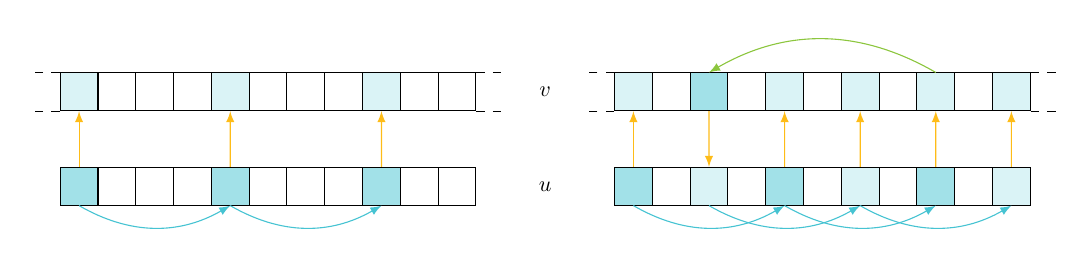
\begin{tikzpicture}[scale=0.8,every node/.style={scale=0.8}]
				
		\foreach \i in {1,...,11} {
			\pgfmathsetmacro{\x}{0.6 * \i}
			\node [draw,rectangle,minimum size=.6cm] (v\i) at (\x cm,0) {};
			\node [draw,rectangle,minimum size=.6cm] (u\i) at (\x cm,-1.5) {};
		}
		
		\node at (8cm,0) {$v$};
		\node at (8cm,-1.5) {$u$};
		
		
		\draw [dashed] (v1.north west) -- ++(-.5,0);
		\draw [dashed] (v1.south west) -- ++(-.5,0);		
		\draw [dashed] (v11.north east) -- ++(.5,0);
		\draw [dashed] (v11.south east) -- ++(.5,0);
		
		\path [color=D3,-{latex}] (u1) edge (v1);
		\path [color=D3,-{latex}] (u5) edge (v5);
		\path [color=D3,-{latex}] (u9) edge (v9);
		
		\path [color=D4,-{latex}] (u1.south) edge [bend right] (u5.south);
		\path [color=D4,-{latex}] (u5.south) edge [bend right] (u9.south);
		%\path [color=C5,-{latex}] (v9.north) edge [bend right] (v3.north);
		
		\begin{pgfonlayer}{background}
			\node [fill,color=D4bg,minimum size=.6cm] at (u1) {};
			\node [fill,color=D4bg,minimum size=.6cm] at (u5) {};
			\node [fill,color=D4bg,minimum size=.6cm] at (u9) {};
			\node [fill,color=D4hint,minimum size=.6cm] at (v1) {};
			\node [fill,color=D4hint,minimum size=.6cm] at (v5) {};
			\node [fill,color=D4hint,minimum size=.6cm] at (v9) {};	
		\end{pgfonlayer}
		
		
		\begin{scope}[shift={(8.8cm,0)}]
			\foreach \i in {1,...,11} {
				\pgfmathsetmacro{\x}{0.6 * \i}
				\node [draw,rectangle,minimum size=.6cm] (v\i) at (\x cm,0) {};
				\node [draw,rectangle,minimum size=.6cm] (u\i) at (\x cm,-1.5) {};
			}
			
			\draw [dashed] (v1.north west) -- ++(-.5,0);
			\draw [dashed] (v1.south west) -- ++(-.5,0);		
			\draw [dashed] (v11.north east) -- ++(.5,0);
			\draw [dashed] (v11.south east) -- ++(.5,0);
			
			\path [color=D3,-{latex}] (u1) edge (v1);
			\path [color=D3,-{latex}] (u5) edge (v5);
			\path [color=D3,-{latex}] (u9) edge (v9);
			
			\path [color=D3,-{latex}] (v3) edge (u3);
			\path [color=D3,-{latex}] (u7) edge (v7);
			\path [color=D3,-{latex}] (u11) edge (v11);
			
			\path [color=D4,-{latex}] (u1.south) edge [bend right] (u5.south);
			\path [color=D4,-{latex}] (u5.south) edge [bend right] (u9.south);
			
			\path [color=C5,-{latex}] (v9.north) edge [bend right] (v3.north);
			
			\path [color=D4,-{latex}] (u3.south) edge [bend right] (u7.south);
			\path [color=D4,-{latex}] (u7.south) edge [bend right] (u11.south);
	
			\begin{pgfonlayer}{background}
				\node [fill,color=D4bg,minimum size=.6cm] at (u1) {};
				\node [fill,color=D4bg,minimum size=.6cm] at (u5) {};
				\node [fill,color=D4bg,minimum size=.6cm] at (u9) {};
				\node [fill,color=D4hint,minimum size=.6cm] at (v1) {};
				\node [fill,color=D4hint,minimum size=.6cm] at (v5) {};
				\node [fill,color=D4hint,minimum size=.6cm] at (v9) {};	
				
				\node [fill,color=D4bg,minimum size=.6cm] at (v3) {};
				\node [fill,color=D4hint,minimum size=.6cm] at (u3) {};
				\node [fill,color=D4hint,minimum size=.6cm] at (v7) {};
				\node [fill,color=D4hint,minimum size=.6cm] at (u7) {};
				\node [fill,color=D4hint,minimum size=.6cm] at (v11) {};
				\node [fill,color=D4hint,minimum size=.6cm] at (u11) {};
			\end{pgfonlayer}
		\end{scope}
		
	\end{tikzpicture}
\end{document}

	\end{center}
	\caption{Alignment of two periodic words with periods of length $6$ and $4$, respectively. We can conclude that the periodic length is at most $2$.}
	\label{fig:periodic-infixes}
\end{figure}


\begin{corollary}
    \label{powers-infixes:cor}
    Let $u,v \in \Sigma^*$ and $k, \ell \in \Nat$
    such that $k \geq \factorial[p]{\card{u} \times \card{v}}$,
    $\ell \geq \factorial[p]{\card{v} \times \card{u}}$,
    and $u^k \infleq v^\ell$.
    Then, there exists $w \in \Sigma^*$ of size at most
    $\min \set{\card{u}, \card{v}}$ and a $p \in \Nat$
    such that
    $u^k \infleq v^\ell \infleq w^p$.
\end{corollary}

The reason why \kl{periodic words} built using a given period $x \in \Sigma^+$
are interesting for the \kl{infix relation} is that they naturally create
\kl{chains} for the \kl{prefix} and \kl{suffix} relations. Indeed, if $x \in
\Sigma^+$ is a finite word, then $\setof{x^p}{p \in \Nat}$ is a \kl{chain} for
the \kl{infix relation}. Note that in general, the \kl{downwards closure} of a
chain is \emph{not} a chain (see \cref{dw-closure-not-wqo:rem}). However, for the chains generated using periodic
words, the \kl{downwards closure} $\dwset[\infleq]{\setof{x^p}{p \in \Nat}}$ is
a \emph{finite union} of \kl{chains}. Because this set will appear in bigger
equations, we introduce the shorter notation $\intro*\InfPeriodChain{x}$ for
the set of \kl{infixes} of words of the form $x^p$, where $p$ ranges over
$\Nat$.


\begin{remark}
    \label{dw-closure-not-wqo:rem}
    Let $(X,\preceq)$ be a quasi-ordered set, and $L \subseteq X$ be such that $(L,
    \preceq)$ is \kl{well-quasi-ordered}. It is not true in general that
    $(\dwset{L}, \preceq)$ is \kl{well-quasi-ordered}. In the case of $(\Sigma^*,
    \infleq)$ a typical example is to start from an infinite \kl{antichain} $A$,
    together with an enumeration $\seqof{w_i}[i \in \Nat]$ of $A$, and build the language $L
    \defined \setof{ \prod_{i = 0}^n w_i }{ i \in \Nat }$. By definition, $L$ is a
    \kl{chain} for the \kl{infix} ordering, hence \kl{well-quasi-ordered}. However,
    $\dwset[\infleq]{L}$ contains $A$, and is therefore not
    \kl{well-quasi-ordered}. 
\end{remark}

\begin{lemma}
    \label{inf-period-chain:lem}
    Let $x \in \Sigma^+$ be a word, and
    Then $\InfPeriodChain{x}$ is a finite union of \kl{chains}
    for the \kl{infix}, \kl{prefix} and \kl{suffix} relations 
    simultaneously.
\end{lemma}
\begin{proof}
    Let $x \in \Sigma^+$ be a word, and let $P_x$ be the (finite) set 
    of all \kl{prefixes} of $x$, and $S_x$ be the (finite)
    set of all \kl{suffixes} of $x$.
    Assume that $w \in \InfPeriodChain{x}$, then $w = u x^p v$ for some
    $u \in S_x$, $v \in P_x$, and $p \in \Nat$.
    We have proven that
    \begin{equation*}
        \InfPeriodChain{x} \subseteq \bigcup_{u \in P_x} \bigcup_{v \in S_x} u x^* v
        \quad .
    \end{equation*}

    Let us now demonstrate that for all $(u,v) \in S_x \times P_x$, the
    language $u x^* v$ is a \kl{chain} for the \kl{infix}, \kl{suffix} and \kl{prefix} relations.
    To that end,
    let $(u,v) \in S_x \times P_x$ and $\ell, k \in \Nat$ be such that $\ell <
    k$, let us prove that $u x^\ell v \infleq u x^k  v$. Because $v \prefleq
    x$, we know that there exists $w$ such that $vw = x$. In particular,
    $ux^\ell vw = u x^{\ell + 1}$, and because $\ell < k$, we conclude that $u
    x^{\ell + 1} \prefleq u x^k v$. By transitivity, $u x^\ell v \prefleq u x^k
    v$, and \emph{a fortiori}, $u x^\ell v \infleq u x^k v$. 
    Similarly, because $u \suffleq x$,  there exists $w$ such that $wu  = x$, 
    and we conclude that $u x^{\ell} v \suffleq w u x^\ell v = x^{\ell + 1} v \suffleq u x^k v$.
\end{proof}



The following combinatorial lemma connects the property of being
\kl{well-quasi-ordered} to a property of the \kl{periodic lengths} of words in
a language, based on the assumption that some factors can be iterated. It is
the core result that powers the analysis done in the upcoming
\cref{bounded-language:thm,infix-amalgamation:thm}.

\begin{lemma}
    \label{pumping-periods:lem}
    Let $L \subseteq \Sigma^*$ be a language
    that is \kl{well-quasi-ordered} by the \kl{infix relation}.
    Let $k \in \Nat$, $u_1, \cdots, u_{k+1} \in \Sigma^*$,
    and $v_1, \cdots, v_{k} \in \Sigma^+$
    be such that
    $w[\vec{n}] \defined (\prod_{i = 1}^k u_i v_i^{n_i}) u_{k+1}$
    belongs to $L$
    for arbitrarily large values of $\vec{n} \in \Nat^k$.
    Then, 
    there exists $x,y \in \Sigma^+$ of size 
    at most $\max \setof{\card{v_i}}{1 \leq i \leq k}$
    such that 
    one of the following holds for all
    $\vec{n} \in \Nat^{k}$:
    \begin{enumerate}
        \item $w[\vec{n}] \in u_1 \InfPeriodChain{x}$,
        \item $w[\vec{n}] \in \InfPeriodChain{x} u_{k+1}$,
        \item $w[\vec{n}] \in \InfPeriodChain{x} u_i \InfPeriodChain{y}$
            for some $1 \leq i \leq k + 1$.

    \end{enumerate}
\end{lemma}
\begin{proof}
    Note that the result is obvious if $k = 0$, and therefore
    we assume $k \geq 1$ in the following proof.

    Let us construct a sequence of words $\seqof{w_i}[i \in \Nat]$, where $w_i
    \defined w[\vec{n_i}]$ for some well-chosen indices $\vec{n_i} \in \Nat^k$. The goal
    being that 
    if $w[\vec{n_i}]$ is an \kl{infix} of $w[\vec{n_j}]$,
    then it can intersect at most \emph{two} iterated words,
    with an intersection that is long enough to successfully apply
    \cref{periodic-infixes:lem}.
    In order to achieve this,
    let us first define $s$ as the maximal size of a word $v_i$
    ($1 \leq i \leq k$) and $u_j$ ($1 \leq j \leq k+1$).
    Then,
    we consider $\vec{n_0} \in \Nat^k$ such that $\vec{n_0}$ has all 
    its components greater than $\factorial{s}$ and such that
    $w[\vec{n_0}]$ belongs to $L$. 
    Then, we inductively define 
    $\vec{n_{i+1}}$  as the smallest vector of numbers greater than $\vec{n_i}$,
    such that $w[\vec{n_{i+1}}]$ belongs to $L$, 
    and with $\vec{n_i}$ having all components greater than
    $2\card{w[\vec{n_i}]}$.


    Let us assume that $k \geq 2$ in the following proof for symmetry purposes,
    and argue later on that when $k = 1$ the same argument goes through.
    Because $L$ is \kl{well-quasi-ordered} by the \kl{infix relation}, there
    exists $i < j$ such that $w[\vec{n_i}]$ is an \kl{infix} of $w[\vec{n_j}]$.
    Now, because of the chosen values for $\vec{n_j}$, there exists $1 \leq \ell \leq
    k-1$ such that $w[\vec{n_i}]$ is actually an \kl{infix} of $u_{\ell}
    v_{\ell}^{n_{j,\ell}} u_{\ell+1} v_{\ell+1}^{n_{j,\ell+1}} u_{\ell+2}$.
    Even more,
    one of the three following equations holds:
    \begin{itemize}
        \item $w[\vec{n_i}] \infleq v_{\ell}^{n_{j,\ell}} u_{\ell+1} v_{\ell+1}^{n_{j,\ell+1}}$,
        \item $w[\vec{n_i}] \infleq u_{\ell}
            v_{\ell}^{n_{j,\ell}}$,
        \item $w[\vec{n_i}] \infleq
            v_{\ell+1}^{n_{j,\ell+1}} u_{\ell+2}$.
    \end{itemize}
    In all those cases, we conclude using \cref{powers-infixes:cor}
    that there exists $x,y \in \Sigma^+$ of size at most $s$, and 
    a number $1 \leq t \leq k$ such that
    $v_i^{n_i} \in \InfPeriodChain{x}$ for all $1 \leq i \leq t$,
    and
    $v_i^{n_i} \in \InfPeriodChain{y}$ for all $t < i \leq k$.
    In particular,
    $w[\vec{n_i}] \in \InfPeriodChain{x} u_{t} \InfPeriodChain{y}$.

    
    When $k = 1$, the situation is a bit more specific since we only have two
    cases: either $w_i \infleq u_1 v_1^{n_j}$ or $w_i \infleq v_1^{n_j} u_2$,
    and we conclude with an identical reasoning.
\end{proof}

\begin{lemma}
    \label{bounded-language:lem}
    Let $L \subseteq \Sigma^*$ be a \kl{bounded language}
    that is \kl{well-quasi-ordered} by the \kl{infix relation}.
    Then, there exists a finite subset $E \subseteq (\Sigma^*)^3$,
    such that:
    \begin{equation*}
        L \subseteq \bigcup_{(x,u,y) \in E} \InfPeriodChain{x} u \InfPeriodChain{y}
        \quad .
    \end{equation*}
\end{lemma}
\begin{proof}
    Let $w_1, \dots, w_n$ be such that
    $L \subseteq w_1^* \cdots w_n^*$.
    Let us define $m \defined \max \setof{\card{w_i}}{1 \leq i \leq n}$

    Let $w[\vec{k}] \defined w_1^{k_1} \cdots w_n^{k_n}$ be a map from $\Nat^k$
    to $\Sigma^*$. We are interested in the intersection of the image of $w$
    with $L$. Let us assume for instance that for all $\vec{k} \in \Nat^n$,
    there exists $\vec{\ell} \geq \vec{k}$ such that $w[\vec{\ell}] \in L$.
    Then, leveraging \cref{pumping-periods:lem}, we conclude that there exists
    $x,y$ of size at most $\max\setof{\card{w_i}}{1 \leq i \leq n}$ such that
    $w[\vec{k}] \in \InfPeriodChain{x} \cup \InfPeriodChain{x}
    \InfPeriodChain{y}$, and we conclude that $L \subseteq \InfPeriodChain{x}
    \cup \InfPeriodChain{x} \InfPeriodChain{y}$.

    Now, it may be the case that one cannot simultaneously assume that two
    component of the vector $\vec{k}$ are unbounded. In general, given a set $S
    \subseteq \set{1, \dots, n}$ of indices, we say that $S$ is admissible if
    there exists a bound $N_0$ such that for all $\vec{b} \in \Nat^S$, there
    exists a vector $\vec{k} \in \Nat^n$, such that $\vec{k}$ is greater than
    $\vec{b}$ on the $S$ components, and the other components are below the
    bound $N_0$. The language of an admissible set $S$ is the set of words
    obtained by repeating $w_i$ at most $N_0$ times if it is not in $S$
    ($w_i^{\leq N_0}$) and arbitrarily many times otherwise ($w_i^*$).
    Note that $L \subseteq \bigcup_{S \text{ admissible }} L(S)$.

    Now, admissible languages are ready to be pumped according to
    \cref{pumping-periods:lem}. For every admissible language,
    the size of a word that is not iterated is at most
    $N_0 \times m$ by definition, and we conclude that:
    \begin{equation}
        \label{bounded-language:eq}
        L \subseteq 
        \bigcup_{x,y \in \Sigma^{\leq n}}
        \bigcup_{u \in \Sigma^{\leq m \times N_0}}
        \InfPeriodChain{x} u \InfPeriodChain{y}
        \cup
        \InfPeriodChain{x} u
        \cup
        u \InfPeriodChain{x}
        \quad .
    \end{equation}
\end{proof}

\begin{proofof}{bounded-language:thm}
    We apply \cref{bounded-language:lem}, and conclude
    because $\InfPeriodChain{x}$ is a finite union of \kl{chains}
    for the \kl{prefix}, \kl{suffix} and \kl{infix} relations
    (\cref{inf-period-chain:lem}).
\end{proofof}


\begin{corollary}
    \label{ordinal-invariants-bounded:cor}
    Let $L$ be a \kl{bounded language} of $\Sigma^*$
    that is \kl{well-quasi-ordered} by the \kl{infix relation}.
    Then, the \kl{ordinal width} of $L$ less than $\omega^2$,
    its \kl{ordinal height} is at most $\omega$,
    and its \kl{maximal order type} less than $\omega^3$.
    Furthermore, those three bounds are tight.
\end{corollary}
\begin{proof}
  Upper bounds are a direct consequence of \cref{bounded-language:thm},
  and the tightness is witnessed by the 
  languages: 
  $L_k \defined \bigcup_{i = 2}^{k+1} (a b^i a)^* (b a^i b)^*$,
  that are \kl{bounded languages} of $\set{a,b}^*$,
  \kl{well-quasi-ordered} by the \kl{infix relation},
  and have \kl{ordinal width}, \kl{ordinal height} and
  \kl{maximal order type} respectively equal to $k \cdot \omega$, $\omega$ and $k \cdot \omega^2$.
\end{proof}

\section{Infixes and Downwards Closed Languages}
\label{infixes-dwclosed:sec}

Let us now discuss another classical restriction that can be imposed on 
languages when studying \kl{well-quasi-orders}, that of being
\kl{downwards closed}. Indeed, the \cref{infix-embedding:thm}
crucially relies on constructing languages that are \emph{not}
\kl{downwards closed}, and we have shown 
in \cref{dw-closure-not-wqo:rem} that the \kl{downwards closure}
of a \kl{well-quasi-ordered} language is not necessarily
\kl{well-quasi-ordered}.

\subsection{Characterization of Well-Quasi-Ordered Downwards Closed Languages}

An immediate consequence of \cref{bounded-language:thm} is that   if $L$ is a
\kl{bounded language}, then considering $L$ or its \kl{downwards closure}
$\dwset[\infleq]{L}$ is equivalent with respect to being
\kl{well-quasi-ordered} by the \kl{infix relation}, as opposed to
the general case illustrated in \cref{dw-closure-not-wqo:rem}.

\begin{corollary}
    \label{bounded-wqo-dwclosed:cor}
    Let $L$ be a \kl{bounded language} of $\Sigma^*$. Then,
    $L$ is a \kl{well-quasi-order} when endowed with the
    \kl{infix relation} if and only if $\dwset[\infleq]{L}$ is.
\end{corollary}
\begin{proof}
    Because $L \subseteq \dwset[\infleq]{L}$, the right-to-left implication
    is trivial.
    For the left-to-right implication, let us assume that $L$ is a
    \kl{well-quasi-ordered} language for the \kl{infix relation}.
    Then $L$ is included in a finite union 
    of products of \kl{chains}: \todo{reference}
    \begin{equation*}
        L \subseteq \bigcup_{i = 1}^n S_i \cdot P_i \quad .
    \end{equation*}
    Remark that the \kl{downwards closure} of a product of two \kl{chains}
    is a finite union of products of two chains. \todo{reference/proof}.
    As a consequence, we conclude that $\dwset[\infleq]{L}$ is itself included
    in a finite union of products of \kl{chains}.
    Note that this also proves that $\dwset[\infleq]{L}$ is a \kl{bounded language},
    hence that it is \kl{well-quasi-ordered} by the \kl{infix relation} 
    via
    \cref{bounded-language:thm}.
\end{proof}

One may think that all \kl{downwards closed} languages for the \kl{infix
relation} that are \kl{well-quasi-ordered} are \kl(language){bounded}. Note
that this is what happens in the case of the \kl{subword embedding}, where any
\kl{downwards closed} language for this relation is characterized by finitely
many excluded \kl{subwords}, hence provides a \kl{bounded language} \todo{wrong? $\{a,b\}^*$ is downward closed but not bounded}. However, this
is not the case for the \kl{infix relation}, as we will now illustrate with the
following two examples.

\begin{example}
    \label{dwclosed-wqo-not-finite-excl:ex}
    Let $L \defined a^* b^* \cup b^* a^*$ \todo{However, this language is bounded, so this seems to be a non sequitur}. This language is \kl{downwards
    closed} for the \kl{infix relation}, is \kl{well-quasi-ordered} for the
    \kl{infix relation}, but is characterized by an \emph{infinite} number 
    of excluded infixes, respectively of the form $ab^ka$ and $ba^kb$ where $k \geq 1$.
\end{example}

To strengthen \cref{dwclosed-wqo-not-finite-excl:ex}, we will
leverage the \intro{Thue-Morse sequence} $\intro*\ThueMorse \in
\set{0,1}^{\Nat}$, which we will use as a black-box for its two main
characteristics: it is \kl{cube-free} and \kl{uniformly recurrent}. Being
\intro{cube-free} means that no (finite) word of the form $uuu$ is an
\kl{infix} of $\ThueMorse$, and being \intro{uniformly recurrent} means that
for every word $u$ that is an \kl{infix} of $\ThueMorse$, there exists $k \geq
1$ such that $u$ is an \kl{infix} of every word $v$ of size at least $k$. We
refer the reader to a nice survey of Allouche and Shallit for more information
on this sequence and its properties \cite{ALSHA99}.

\begin{theorem}
    \label{uniformly-recurrent:lem}
    Let $w \in \Sigma^\Nat$ be a \kl{uniformly recurrent} word.
    Then, the set of finite \kl{infixes} of $w$ is \kl{well-quasi-ordered} for the \kl{infix relation}.
\end{theorem}
\begin{proof}
    Let $L$ be the set of finite \kl{infixes} of $w$.
    Consider a sequence $\seqof{u_i}[i \in \Nat]$ of words in $L$. Without loss of
    generality, we may consider a subsequence such that $\card{u_i} <
    \card{u_{i+1}}$ for all $i \in \Nat$. Because $\ThueMorse$ is \kl{uniformly
    recurrent}, there exists $k \geq 1$ such that $u_1$ is an \kl{infix} of
    every word $v$ of size at least $k$. In particular, $u_1$ is an \kl{infix}
    of $u_k$, hence the sequence $\seqof{u_i}[i \in \Nat]$ is \kl(sequence){good}.
\end{proof}


\begin{lemma}
    \label{thue-morse:lemma}
    The language $\intro*\LMorse$ of \kl{infixes} of the \kl{Thue-Morse sequence}
    is \kl{downwards closed} for the \kl{infix
    relation}, \kl{well-quasi-ordered} for the \kl{infix relation}, but is not
    \kl(language){bounded}.
\end{lemma}
\begin{proof}
    By construction $\LMorse$ is an \emph{infinite}
    \kl{downwards closed} for the \kl{infix relation}. Let us argue that $\LMorse$ is
    \kl{well-quasi-ordered} for the \kl{infix relation}, but is not \kl(language){bounded}.
    It is \kl{well-quasi-ordered} because it is the set of finite \kl{infixes}
    of a \kl{uniformly recurrent} word, and we can apply \cref{uniformly-recurrent:lem}.

    Assume by contradiction that $\LMorse$ is \kl(language){bounded}. In this case, there exist
    words $w_1, \dots, w_k \in \Sigma^*$ such that $L \subseteq w_1^* \cdots
    w_k^*$. Since $L$ is infinite and \kl{downwards closed}, there exists a
    word $u \in L$ such that $u = w_i^3$ for some $1 \leq i \leq k$. This is absurd
    because $u \infleq \ThueMorse$, which is \kl{cube-free}.
\end{proof}

One may refine our analysis of the \kl{Thue-Morse sequence} to obtain 
precise bounds on the \kl{ordinal invariants} of its language of \kl{infixes}.

\begin{lemma}
    \label{thue-morse-ordinal:lemma}
    The \kl{maximal order type} of $\LMorse$ is $\omegaOrd$,
    the \kl{ordinal height} of $\LMorse$ is $\omegaOrd$,
    the \kl{ordinal width} of $\LMorse$ is $\omegaOrd$.
\end{lemma}
\begin{proof}
    Let us prove that these are upper bounds for the \kl{ordinal invariants} of
    $L$. For the \kl{ordinal height}, it is true for any language $\LMorse$.
    For the \kl{maximal order type}, we remark that
    the maximal length of a \kl{bad sequence} is determined by its first element,
    hence that it is at most $\omegaOrd$.
    Finally, because the \kl{ordinal width} is at most the \kl{maximal order type},
    we conclude that the \kl{ordinal width} is also at most $\omegaOrd$.

    Now, let us prove that these bounds are tight. It is clear that
    $\oHeight{\LMorse} = \omegaOrd$: given any number $n \in \Nat$, one can construct a
    \kl{decreasing sequence} of words in $L$ of length $n$, for instance by
    considering the first $n$ prefixes of the \kl{Thue-Morse sequence} by
    decreasing size.
    Let us now prove that $\oWidth{\LMorse} = \omegaOrd$. Assume by contradiction that
    $\oWidth{\LMorse}$ is finite. Then, $L$ can be written as a finite union of
    \kl{chains} for the \kl{infix relation}, and in particular, $L$ is
    \kl(language){bounded}, which is absurd by \cref{thue-morse:lemma}.
    Finally, because the \kl{ordinal width} is at most the \kl{maximal order
    type}, we conclude that the \kl{maximal order type} of $\LMorse$ is also $\omegaOrd$.
\end{proof}


We prove if the upcoming theorem that the status of the \kl{Thue-Morse
sequence} is actually representative of most \kl{downwards closed} languages
for the \kl{infix relation}. Indeed, we show that the \kl{ordinal invariants}
of such languages are relatively small, and the proof of this fact relies on
the connection between \kl{well-quasi-ordered} languages and \kl{uniformly
recurrent} words.

\begin{theorem}
    \label{small-ordinal-invariants:thm}
    Let $L$ be a \kl{well-quasi-ordered} language for the \kl{infix relation}
    that is \kl{downwards closed}.
    Then, the \kl{maximal order type} of $L$ is strictly less than $\omegaOrd^3$,
    its \kl{ordinal height} is at most $\omegaOrd$,
    and its \kl{ordinal width} is at most $\omegaOrd^2$.

    Furthermore, those bounds are tight.
\end{theorem}

\AP A subset $I \subseteq X$ is \intro(subset){directed} if, for every $x,y \in
I$, there exists $z \in I$ such that $x \leq z$ and $y \leq z$. Given a
\kl{well-quasi-order} $(X, \leq)$, one can always decompose $X$ into a finite
union of \intro{order ideals}, that is, non-empty sets $I \subseteq X$ that are
\kl{downwards closed} and \kl(subset){directed} for the relation $\leq$. In our
case, a \kl{well-quasi-ordered} \kl{order ideal} for the \kl{infix relation} is
the set of finite \kl{infixes} of a finite or bi-infinte word $w \in
\Sigma^\Nat \cup \Sigma^\Rel $ (\cref{bi-infinite:lem}). Therefore, we will
first study languages that are described as the set of finite \kl{infixes} of
some (bi-)infinite word (\cref{ultimately-uniformly-recurrent:lem}). To that
end, let us introduce the notation $\intro*\infset{w}$ for the set of finite
\kl{infixes} of a (possibly infinite or bi-infinite) word $w$.

\begin{lemma}
    \label{bi-infinite:lem}
    Let $L \subseteq \Sigma^*$ be an \kl{order ideal} that is \kl{well-quasi-ordered} 
    for the 
    \kl{infix relation}. Then $L$ is the set of finite \kl{infixes}
    of a finite, infinite or bi-infinite word $w$.
\end{lemma}
\begin{proof}
    Let us assume that $L$ is infinite, the case when it is finite 
    is similar, but leads to a finite word.

    Because the alphabet $\Sigma$ is finite, we can enumerate the words of $L$
    as $\seqof{w_i}[i \in \Nat]$. Now, let us build the sequence $\seqof{u_i}[i \in \Nat]$ by induction
    as follows: $u_0 = w_0$, and $u_{i+1}$ is a word that contains $u_i$ and
    $w_i$, which exists in $L$ because $L$ is \kl(subset){directed}. Since $L$ is
    \kl{well-quasi-ordered}, one can extract an infinite set of indices $I
    \subseteq \Nat$ such that $u_i \infleq u_{j}$ for all $i \leq j \in I$.

    We can build a word $w$ as the limit of the sequence $\seqof{u_i}[i \in
    I]$. This word is infinite or bi-infinite, and contains as infixes all the
    words $u_i$ for $i \in I$. Because every word of $L$ is an infix of every
    $u_i$ for a large enough $I$, one concludes that $L$ is contained in the
    set of finite infixes of $w$. Conversely, every finite infix of $w$ is 
    an infix of some $u_i$ by definition of the limit construction, hence
    belongs to $L$ since $u_i \in L$ and $L$ is \kl{downwards closed}.
\end{proof}


\AP We say that an infinite word $w \in \Sigma^\Nat$ is \intro{ultimately
uniformly recurrent} if there exists a bound $N_0 \in \Nat$ such that $w_{\geq
N_0}$ is \kl{uniformly recurrent}.

\begin{lemma}
    \label{ultimately-uniformly-recurrent:lem}
    Let $w \in \Sigma^\Nat$ be an infinite word. 
    Then, the set of finite infixes of $w$ is \kl{well-quasi-ordered} for the \kl{infix relation}
    if and only if $w$ is \kl{ultimately uniformly recurrent}.
\end{lemma}
\begin{proof}

    Assume that $w$ is \kl{ultimately uniformly recurrent}. Consider a sequence
    of words $\seqof{w_i}[i \in \Nat]$ that are finite \kl{infixes} of $w$. Because $w$ is
    \kl{ultimately uniformly recurrent}, there exists a bound $N_0$ such that
    $w_{\geq N_0}$ is \kl{uniformly recurrent}. Let $i < N_0$, we claim that,
    without loss of generality, only finitely many words in the sequence
    $\seqof{w_i}[i \in \Nat]$ can be found starting at the position $i$ in $w$. Indeed, if
    it is not the case, then we have an infinite subsequence of words that are
    all comparable for the \kl{infix relation}, and therefore a \kl{good
    sequence}, because the \kl{infix relation} is \kl{well-founded}. We can
    therefore assume that all words in the sequence $\seqof{w_i}[i \in \Nat]$ are such that
    they start at a position $i \geq N_0$. But then, they are all finite
    \kl{infixes} of $w_{\geq N_0}$, which is a \kl{uniformly recurrent} word,
    whose set of finite \kl{infixes} is \kl{well-quasi-ordered}
    (\cref{uniformly-recurrent:lem}).

    Conversely, assume that the set of finite infixes of $w$ is
    \kl{well-quasi-ordered}. Let us write $\mathsf{Rec}(w)$ the set of finite
    \kl{infixes} of $w$ that appear infinitely often. We can similarly define
    $\mathsf{Rec}(w_{\geq i})$ for any (infinite) suffix of $w$. The sequence
    $R_i \defined \mathsf{Rec}(w_{\geq i})$ is a sequence of \kl{downwards
    closed} sets of finite words, included in the set of finite infixes of $w$
    by definition. Because the latter is \kl{well-quasi-ordered}, there exists
    an $N_0 \in \Nat$, such that $\bigcap_{i \in \Nat} R_i = R_{N_0}$.
    Now, consider $v \defined w_{\geq N_0}$. By construction, 
    every finite infix of $v$ 
    appears infinitely often in $v$. Let us consider 
    some finite infix $u \infleq v$, we claim that there is a bound $N_u$
    on the distance
    between two consecutive occurrences of $u$ in $v$.
    Indeed, if it is not the case, then there exists an infinite sequence
    $\seqof{u x_i u}[i \in \Nat]$ of infixes of $v$, such that $x_i$ is a word that is
    of size $\geq i$.
    Because the finite infixes of $w$ (hence, of $v$) are \kl{well-quasi-ordered},
    one can extract an infinite set of indices $I \subseteq \Nat$
    such that $u x_i u \infleq u x_{j} u$ for all $i \leq j \in I$.
    In particular, $u x_i u \infleq u x_{j} u$ for some $j > |x_i|$, 
    which contradicts the fact that $u x_j u$ coded two consecutive
    occurrences of $u$ in $v$.

    We have shown that for every finite infix $u$ of $v$, there exists a bound
    $N_u$ such that every two occurrences of $u$ in $v$ start at distance at
    most $N_u$. In particular, there exists a bound $M_u$ such that every infix
    of $v$ of size at least $M_u$ contains $u$. We have proven that
    $v$ is \kl{uniformly recurrent}, hence that $w$ is \kl{ultimately uniformly
    recurrent}.
\end{proof}

\begin{lemma}
    \label{small-ordinal-invariants:lem}
    Let $w \in \Sigma^\Nat$ be an \kl{ultimately uniformly recurrent} word.
    Then, the set of finite infixes of $w$ has \kl{ordinal width}
    less than $2 \cdot \omegaOrd$.
    Furthermore, this bound is tight. 
\end{lemma}
\begin{proof}
    Let $N_0$ be a bound such that $w_{\geq N_0}$ is \kl{uniformly recurrent}.
    Let us write $\infset{w}$ the set of finite infixes of $w$.
    We prove that $\oWidth{\infset{w}} \leq \omegaOrd + N_0$.
    Let $u_1 \infleq w$ be a finite word. 

    If $u_1$ is an \kl{infix} of $w_{\geq N_0}$, then there exists $k \geq 1$
    such that $u_1$ is an \kl{infix} of every word of size at least $k$. In
    particular, there is finite bound on the length of every sequence of
    incomparable elements starting with $u_1$. We conclude in particular that
    $\infset{w} \setminus \upset{u_1}$ has a finite \kl{ordinal width}.

    Otherwise, $u_1$ can only be found \emph{before} $N_0$. In this case, we
    consider a second element of a \kl{bad sequence} $u_2 \infleq w$, which is
    incomparable with $u_1$ for the \kl{infix relation}. If $u_2$ is an
    \kl{infix} of $w_{\geq N_0}$, then we can conclude as before. Otherwise,
    notice that $u_1$ and $u_2$ cannot start at the same position in $w$
    (because they are incomparable). Continuing this argument, we conclude that
    there are at most $N_0$ elements starting before $N_0$
    at the start of any sequence of
    incomparable elements in $\infset{w}$. We conclude that
    $\oWidth{\infset{w}} \leq \omegaOrd + N_0$.

  Let us now justify that this bound is tight.
  The \kl{Thue-Morse sequence} over a binary
  alphabet $\set{a,b}$ has \kl{ordinal width} $\omegaOrd$
  from \cref{thue-morse-ordinal:lemma}.
    Given a number $N_0
  \in \Nat$, one can construct an arbitrarily long \kl{antichain} of words for
  the \kl{infix relation} by using a new letter $c$. When concatenating this
  (finite) antichain as a prefix of the \kl{Thue-Morse sequence}, one obtains a
  new (infinite) word $w$. It is clear that the \kl{ordinal width} of
  $\infset{w}$ is now at least $\omegaOrd + N_0$.
\end{proof}


The behaviour of bi-infinite words is very similar to the behaviour of infinite
ones. Given a bi-infinite word $w \in \Sigma^{\Rel}$, we can consider $w_+ \in
\Sigma^\Nat$ and $w_- \in \Sigma^\Nat$ the two infinite words obtained as
follows: for all $i \in \Nat$, $(w_+)_i = w(i)$ and $(w_-)_i = w(-i)$. Note
that the two share the letter at position $0$.

\begin{lemma}
    \label{from-bi-to-single:lem}
    Let $w \in \Sigma^\Rel$ be a bi-infinite word. Then, the set of finite
    infixes of $w$ is \kl{well-quasi-ordered} for the \kl{infix relation} if
    and only if $w_+$ and $w_-$ are two \kl{ultimately uniformly recurrent}
    words. In this case, the \kl{ordinal width}
    of the set of finite infixes of $w$ is less than $3 \cdot \omegaOrd$,
    and this bound is tight.
\end{lemma}
\begin{proof}
    Assume that $w_+$ and $w_-$ are \kl{ultimately uniformly recurrent}. Let us
    write $\infset{w}$ the set of finite infixes of $w$. Consider an infinite
    sequence of words $\seqof{u_i}[i \in \Nat]$ in $\infset{w}$. If there is an
    infinite subsequence of words that are all in $\infset{w_+}$, then there
    exists an increasing pair of indices $i < j$ such that $u_i \infleq
    u_j$ because \cref{uniformly-recurrent:lem} applies to $w_+$. Similarly, if
    there is an infinite subsequence of words that are all in $\infset{w_-}$,
    then there exists an increasing pair of indices $i < j$ such that $u_i
    \infleq u_j$ because \cref{uniformly-recurrent:lem} applies to $w_-$ (and
    the \kl{infix relation} is compatible with mirroring). Otherwise, one can
    assume without loss of generality that all words in the sequence have a
    starting position in $w_-$ and an ending position in $w_+$. In this case,
    let us write $(k_i,l_i) \in \Nat^2$ the pair of indices such that $u_i$ is the infix
    of $w$ that starts at position $-k_i$ of $w$ (i.e., $k_i$ of $w_-$) and
    ends at position $l_i$ of $w$ (i.e., $l_i$ of $w_+$).
    Because $\Nat^2$ is a \kl{well-quasi-ordering} with the product ordering,
    there exists $i < j$ such that $k_i \leq k_j$ and $l_i \leq l_j$, 
    in particular, $u_i \infleq u_j$. We have proven that every infinite
    sequence of words in $\infset{w}$ is \kl(wqo){good}, hence $\infset{w}$ is
    \kl{well-quasi-ordered}.

    Conversely, assume that $\infset{w}$ is \kl{well-quasi-ordered}. In
    particular, the subset $\infset{w_+} \subseteq \infset{w}$ is \kl{well-quasi-ordered}.
    Similarly, $\infset{w_-}$ is \kl{well-quasi-ordered} because the \kl{infix
    relation} is compatible with mirroring. Applying
    \cref{ultimately-uniformly-recurrent:lem}, we conclude that both are
    \kl{ultimately uniformly recurrent} words.

    To obtain the upper bound of $3 \cdot \omegaOrd$, we can consider the same
    argument as for \cref{small-ordinal-invariants:lem}. We let $N_0$ be such
    that $w_{\geq N_0}$ and $(w_-)_{\geq N_0}$ are \kl{uniformly recurrent}
    words. In any sequence of incomparable elements of $\infset{w}$, there are
    less than $N_0^2$ elements that are found in $(w_{< N_0})_{> -N_0}$. Then,
    one has to pick a finite \kl{infix} in either $w_{\geq N_0}$ or $w_{\leq
    -N_0}$. Because of \cref{small-ordinal-invariants:lem}, any sequence of
    incomparable elements of these two infinite words has length bounded based
    on the choice of the first element of that sequence. This means that the
    \kl{ordinal width} of $\infset{w}$ is at most $\omegaOrd + \omegaOrd +
    N_0^2$. We conclude that $\oWidth{\infset{w}} < 3 \cdot \omegaOrd$.

  Let us briefly argue that the bound is tight. Indeed, one can
  construct a bi-infinite word $w$ by concatenating a reversed \kl{Thue-Morse
  sequence} on a binary alphabet $\set{a,b}$, a finite antichain of arbitrarily
  large size over a distinct alphabet $\set{c,d}$, and then a \kl{Thue-Morse
  sequence} on a binary alphabet $\set{e,f}$. The \kl{ordinal width} of the set
  of \kl{infixes} of $w$ is then at least $2 \cdot \omegaOrd + K$, where $K$ is the
  size of the chosen antichain, following the same argument as in the proof of
  \cref{small-ordinal-invariants:lem}, using \cref{thue-morse-ordinal:lemma}.
\end{proof}

We are now ready to conclude the proof of \cref{small-ordinal-invariants:thm}.
\begin{proofof}{small-ordinal-invariants:thm}
    It is always true that the \kl{ordinal height} of a language over a finite
    alphabet is at most $\omegaOrd$. Let us now consider a
    \kl{well-quasi-ordered} language $L$ that is \kl{downwards closed} for the
    \kl{infix relation}. Because it is a \kl{well-quasi-ordered} set, it can be
    written as a finite union of \kl{order ideals} $L = \bigcup_{i = 1}^n L_i$.

    For every such \kl(order){ideal} $L_i$, we can apply
    \cref{bi-infinite:lem}, and conclude that $L_i$ is the set of finite
    \kl{infixes} of a finite, infinite or bi-infinite word $w_i$. We can then
    directly conclude that $\oWidth{L_i}$ less than $\omegaOrd$ (in the case of
    a finite word), less than $2 \cdot \omegaOrd$ (in the case of an infinite
    word thanks to \cref{small-ordinal-invariants:lem}), or less than $3 \cdot
    \omegaOrd$ (in the case of a bi-infinite word, thanks to
    \cref{from-bi-to-single:lem}). In any case,
    we have the bound $\oWidth{L_i} < 3 \cdot \omegaOrd$.

    Now, $\oWidth{L} \leq \sum_{i = 1}^n \oWidth{L_i} < 3 \cdot \omegaOrd <
    \omegaOrd^2$. We conclude that the \kl{ordinal width} of $L$ is less than
    $\omegaOrd^2$. Finally, the inequality $\oType{L} \leq \oWidth{L} \oComProd
    \oHeight{L} < \omega \oComProd \omega^2 = \omegaOrd^3$ allows us to conclude.

    The tightness of the bounds is a direct consequence of
    \cref{from-bi-to-single:lem}, and by considering a finite union of 
    these examples over disjoint alphabets (or even, by considering a binary 
    alphabet and using unambiguous codes to separate the different components).
\end{proofof}

\subsection{Decision Procedures}
\label{decision-procedures:sec}

\AP As we have demonstrated, infinite (or bi-infinite words) can be used to
represent languages that are \kl{well-quasi-ordered} for the \kl{infix
relation} by considering their set of finite \kl{infixes}.
Let us formalise the representation of languages by sets of bi-infinite
words that we will use in this section, following the characterization of
\cref{bi-infinite:lem}. A \intro{sequence representation} of a language $L
\subseteq \Sigma^*$ is a finite set of triples $(w_i^-, a_i, w_i^+)_{1 \leq i
\leq n}$ where $w_i^-, w_i^+ \in \Sigma^\Nat \cup \Sigma^*$ are two potentially
infinite words, and $a_i \in \Sigma$ is a letter, such that
\begin{equation*}
    L = \bigcup_{i = 1}^n \infset{\mathsf{reversed}(w_i^-) a_i w_i^+} \quad .
\end{equation*}

\AP Given an effective representation of sequences, one obtains an effective
representation of languages via \kl{sequence representations}. In this section,
we will rely on definitions originating from the area of symbolic dynamics,
that precisely study infinite words whose generation follows from a finitely
described process. However, we will not assume that the reader is familiar with
this domain, and we will use as black-boxes key results from this area.

\AP A first model that one can use to represent infinite words is the model of
\intro{automatic sequences}. In this case, the infinite word $w$ is described
by a finite state automaton, that can compute the $i$-th letter of the word $w$
given as input the number $i$ written in some base $b \in \Nat$. An example of
such a sequence is the \kl{Thue-Morse sequence} that can be described by a
finite automaton using a binary representation of the indices. The good
algorithmic properties of \kl{automatic sequences} come from the fact that a
Presburger definable property that uses letters of the sequence can be
(trivially) translated into a finite automaton that reads the base $b$
representation of the free variables (that are indices of the sequence). We
briefly explain in the following lemma the folklore result that one can decide
if an \kl{automatic sequence} is \kl{ultimately uniformly recurrent}.

\begin{lemma}
  \label{automatic-uur:lem}
    Given an \kl{automatic sequence} $w \in \Sigma^{\Nat}$, one can decide
    whether it is \kl{ultimately uniformly recurrent}.
\end{lemma}
\begin{proof}
    We can rewrite this as a question on the \kl{automatic sequence} $w$
    as follows:
    \begin{align*}
        &\exists N_0,                   &   \text{ultimately} \\
        &\forall i_s \geq N_0,          &   \text{for every infix (start) } u \\
        &\forall i_e > i_s,             &   \text{for every infix (end) }   u \\
        &\exists k \geq 1,              &   \text{there exists a bound} \\
        &\forall j_s \geq N_0,          &   \text{for every other infix (start) } v \\
        &\forall j_e \geq j_s + k,      &   \text{of size at least $k$} \\
        &\exists l \geq 0,              &   \text{there exists a position in } v \\
        &\forall 0 \leq m < i_e - i_s,  &   \text{where } u \text{ can be found} \\
        &j_s + m + l < j_e \land
        w(i_s + m) = w(j_s + m + l) \quad .
    \end{align*}
    Because $w$ is computable by a finite automaton, one can reduce the above
    formula to a regular language, for which it suffices to check emptiness, which
    is decidable.
\end{proof}

Based on \cref{automatic-uur:lem}, we can now prove the following theorem.
\begin{theorem}
    \label{automatic-wqo:thm}
    Given a \kl{sequence representation} of a language $L \subseteq
    \Sigma^*$ where all infinite words are \kl{automatic sequences}, one can
    decide whether $L$ is \kl{well-quasi-ordered} for the \kl{infix relation}.
\end{theorem}
\begin{proof}
    It is easy to see that $L$ is \kl{well-quasi-ordered} for the \kl{infix
    relation} if and only if for every triple $(w_i^-, a_i, w_i^+)$ in the
    \kl{sequence representation} of $L$, the (potentially bi-infinite) word
    $\mathsf{reversed}(w_i^-) a_i w_i^+$ defines a \kl{well-quasi-ordered}
    language. By \cref{from-bi-to-single:lem}, this is the case if and only if
    both $w_i^-$ and $w_i^+$ are \kl{ultimately uniformly recurrent}. 
    Since one can decide whether an \kl{automatic sequence} is
    \kl{ultimately uniformly recurrent} using \cref{automatic-uur:lem},
    we conclude the proof.
\end{proof}


\AP In fact, \kl{automatic sequences} are part of a larger family of sequences
studied in symbolic dynamics, called \kl{morphic sequences}. Let us first
recall that a \intro(words){morphism} is a function $f \colon \Sigma^* \to
\Gamma^*$ such that for every $u,v \in \Sigma^*$, $f(uv) = f(u)f(v)$. A
\intro{morphic sequence} $w$ is an infinite word obtained by iterating a
\kl(words){morphism} $f \colon \Sigma^* \to \Sigma^*$ on a letter $a \in
\Sigma$ such that $f(a)$ starts with $a$, and then applying a
\kl(words){homomorphism} $h \colon \Sigma^* \to \Gamma^*$. The infinite word
$f^\omega(a)$ is the limit of the sequence $\seqof{f^n(a)}[n \in \Nat]$, which
is well-defined because $f(a)$ starts with $a$, and the \kl{morphic sequence}
is $ w \defined h(f^\omega(a))$. 

\AP
Every \kl{automatic
sequence} is a \kl{morphic sequence}, but not the other way around. We refer
the reader to a short survey of \cite{ALSZ17} for more details on the possible
variations on the definition of \kl{morphic sequences} and their relationships.
It was relatively recently proven that one can decide whether a \kl{morphic
sequence} is \kl{uniformly recurrent} \cite[Theorem 1]{DURAND13}. We were not
able to find in the literature whether one can decide \kl{ultimate uniform
recurrence}, but we can prove it for a restricted class of \kl{morphic
sequences}, that are called \intro{pure morphic sequences}, and are precisely
those that do not use a final \kl(words){homomorphism} $h$. Following the same proof
as for \cref{automatic-wqo:thm}, one deduces from the upcoming
\cref{morphic-uur:lem} the following \cref{morphic-wqo:cor}. We actually
conjecture that \cref{morphic-uur:lem} can be extended to all \kl{morphic
sequences} \cref{morphic-uur:conj}.

\begin{lemma}
  \label{morphic-uur:lem}
    Given a \kl{pure morphic sequence} $w \in \Sigma^{\Nat}$, one can decide
    whether it is \kl{ultimately uniformly recurrent}.
\end{lemma}
\begin{proof}
  On the one hand, one can guess a bound $N_0$ and check that 
  the suffix of the word $w_{\geq N_0}$ is \kl{uniformly recurrent},
  since the suffix of a \kl{morphic sequence} is also a \kl{morphic sequence},
  and \kl{uniform recurrence} is decidable for \kl{morphic sequences}
  \cite[Theorem 2]{DURAND13}.

  Let us now prove that a specific choice of $N_0$ is sufficient. Let us write
  $w \defined f^\omega(a)$ where $f \colon \Sigma^* \to \Sigma^*$ is a
  \kl(words){morphism} and $a \in \Sigma$ is a letter such that $f(a)$ starts
  with $a$. Let us also write $f(a) = a s$, where $s \in \Sigma^+$ is a
  non-empty word. Notice that $w = a s f(s) f^2(s) \cdots$. Without loss of
  generality, one can assume that $|f^n(s)| \to \infty$ when $n \to \infty$,
  otherwise $w$ is ultimately periodic, and therefore \kl{ultimately uniformly
  recurrent}. Since one can algorithmically detect if this is the case, we
  assume that it is not.

  Because $\Sigma$ is finite, there exists a finite set of letters $A \subseteq
  \Sigma$ and a suffix $w'$ of $w$ such that $w' \in A^*$ and every letter of
  $w'$ appears infinitely often in $w'$. Furthermore, one can compute this set
  $A$ and a bound $N_0$ such that $f^n(s) \in A^*$ for every $n \geq N_0$. We
  claim that $w$ is \kl{ultimately uniformly recurrent} if and only if
  $f^{N_0}(s) f^{N_0 + 1}(s) \cdots$ is \kl{uniformly recurrent}.
  One direction being obvious, we assume that $w$ is \kl{ultimately uniformly
  recurrent}, and let us prove that $f^{N_0}(s) f^{N_0 + 1}(s) \cdots$ is
  \kl{uniformly recurrent}. 

  Let us assume that $w'' \defined f^{N_1}(s) f^{N_1 + 1}(s) \cdots$ where $N_1
  \geq N_0$ is \kl{uniformly recurrent}. Let us show that $f^{N_0}(s)$ is an
  \kl{infix} of $w''$ if and only if there exists a letter $b$ in $s$ such that
  $f^{N_0}(s) \infleq f^{k} (b)$ for some finite number $k$.

  Assume that $f^{N_0}(s)$ is an \kl{infix} of $w''$. Recall that $|f^n(s)| \to
  \infty$ when $n \to \infty$, hence, there must exist a letter $b$ in $s$ such
  that $|f^n(b)| \to \infty$ when $n \to \infty$. Because every letter of
  $f^{N_0}(s)$ appears infinitely often in $w''$, $f^n(b)$ is a growing
  sequence of infixes of $w''$. Since $w''$ is \kl{uniformly recurrent}, there
  exists a bound $K$ such that $f^{N_0}(s)$ is an \kl{infix} of every $f^k(b)$
  for $k \geq K$. Conversely, if there exists a letter $b$ in $s$ such that
  $f^{N_0}(s) \infleq f^{k} (b)$ for some finite number $k$, then $f^{N_0}(s)$
  is an \kl{infix} of $w''$ because $f^n(b)$ is an infix of $w''$ for every $n
  \in \Nat$.

  Because $w''$ is \kl{uniformly recurrent}, there exists a bound $K$ such that
  $f^{N_1}(s) \infleq f^k(b)$ for every $k \geq K$.
  \todo[inline]{Cannot finish the proof...}

\end{proof}

\begin{corollary}
    \label{morphic-wqo:cor}
    Given a \kl{sequence representation} of a language $L \subseteq
    \Sigma^*$ where all infinite words are \kl{pure morphic sequences}, one can
    decide whether $L$ is \kl{well-quasi-ordered} for the \kl{infix relation}.
\end{corollary} 



\begin{conjecture}
  \label{morphic-uur:conj}
    Given a \kl{morphic sequence} $w \in \Sigma^{\Nat}$, one can decide
    whether it is \kl{ultimately uniformly recurrent}.
\end{conjecture}
